\RequirePackage{luatex85}
\documentclass[border=6pt]{standalone}
\usepackage{tikz}
\usepackage[compat=1.1.0]{tikz-feynman}
\usepackage{amsmath}
\usetikzlibrary{decorations.pathmorphing,decorations.markings,arrows.meta,patterns}

\begin{document}
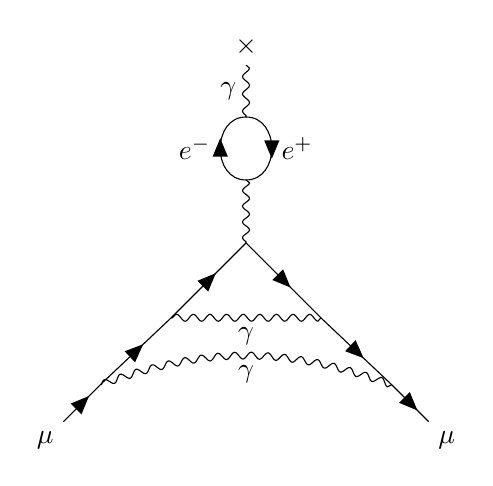
\begin{tikzpicture}
\begin{feynman}
  \vertex at (0, 4.0)  (top) {\(\times\)};
  \vertex at (0, 3.1)  (eL);
  \vertex at (0, 2.3)  (eR);
  \vertex at (0, 1.5)  (vtx);
  \vertex at (-0.95, 0.55) (l1);
  \vertex at ( 0.95, 0.55) (r1);
  \vertex at (-1.85,-0.30) (l2);
  \vertex at ( 1.85,-0.30) (r2);
  \vertex at (-2.55,-1.0) (lmu) {\(\mu\)};
  \vertex at ( 2.55,-1.0) (rmu) {\(\mu\)};
  \diagram* {
    (lmu) -- [fermion] (l2) -- [fermion] (l1) -- [fermion] (vtx) -- [fermion] (r1) -- [fermion] (r2) -- [fermion] (rmu),
    % external photon going up, broken by an e+e- loop
    (vtx) -- [photon] (eR),
    (eR) -- [fermion, half left, edge label=\(e^{-}\), looseness=1.4] (eL),
    (eL) -- [fermion, half left, edge label=\(e^{+}\), looseness=1.4] (eR),
    (eL) -- [photon, edge label=\(\gamma\)] (top),
    % two inner photon arcs across the V
    (l1) -- [photon, edge label'=\(\gamma\)] (r1),
    (l2) -- [photon, edge label'=\(\gamma\), bend left=20] (r2),
  };
\end{feynman}
\end{tikzpicture}
\end{document}
